\chapter{Đọc thêm: Matrix World (Đại số tuyến tính cho mọi người)}
\label{ch:M2L3-reading}

% Nguồn: Hiranabe, Kenji. "Matrix World." \emph{Linear Algebra for Everyone}. March 2023. https://github.com/kenjihiranabe/The-Art-of-Linear-Algebra/blob/main/MatrixWorld.pdf
% Phần cần đọc: Trang 2--4 (~20 phút)
% Nội dung bắt buộc đọc: được kiểm tra trong mọi bài đánh giá (kể cả Quiz).

\section{Thông tin nguồn}

\begin{itemize}
  \item \textbf{Nguồn:} Hiranabe, Kenji. "Matrix World." \emph{Linear Algebra for Everyone}. March 2023. \url{https://github.com/kenjihiranabe/The-Art-of-Linear-Algebra/blob/main/MatrixWorld.pdf}
  \item \textbf{Phần cần đọc:} Trang 2--4 (~20 phút)
\end{itemize}

% [PDF p.2]
\section{Thế giới Ma trận : Bức tranh về Mọi Ma trận}

Tôi rất vui khi được kể lại lịch sử của Thế giới Ma trận (Matrix World) --- tác phẩm sáng tạo của Kenji Hiranabe tại Nhật Bản. Vào tháng 4 năm 2020, bạn của ông là Satomi Joba đã hỏi liệu tôi có thể gửi cho ông một tin nhắn chúc mừng sinh nhật như một bất ngờ hay không. Ông ấy đã rất vui (và vô cùng ngạc nhiên). Kenji kết hợp toán học với nghệ thuật và điện toán: ba tài năng trong một con người. Tôi mới là người phải ngạc nhiên khi ông gửi Thế giới Ma trận ở phiên bản đầu tiên --- không có tên, không có nhiều mục và ý tưởng như bạn thấy bây giờ, nhưng với ý tưởng cốt lõi là trình bày sự đa dạng tuyệt vời của các ma trận.

Kể từ phiên bản đầu tiên đó, Thế giới Ma trận đã phát triển đều đặn. Nó bao gồm mọi thuộc tính (property) phù hợp và mọi phép phân rã (factorization) thể hiện thuộc tính đó. Thật thú vị khi SVD nằm ở vòng tròn ngoài cùng và ma trận đơn vị (identity matrix) nằm ở trung tâm --- nó có tất cả các thuộc tính tốt: ma trận I là ma trận đường chéo (diagonal), đối xứng xác định dương (positive definite symmetric), trực giao (orthogonal), ma trận chiếu (projection), ma trận chuẩn (normal), khả nghịch (invertible) và ma trận vuông (square).

Lek-Heng Lim đã chỉ ra tính hữu dụng của các ma trận M vừa đối xứng vừa trực giao --- những vị vua và cũng là những nữ hoàng. Trị riêng (eigenvalue) của chúng là 1 và -1. Chúng có dạng M = I - 2P (P = ma trận chiếu đối xứng). Có một sự khớp nối hoàn hảo (neat match) giữa tất cả các ma trận M đó và tất cả các không gian con (subspace) của Rn. Bạn có thể thấy điều gì đó thú vị (hoặc thiếu sót điều gì đó) trong Thế giới Ma trận. Chúng tôi hy vọng bạn sẽ thấy! Cảm ơn Kenji.

Gilbert Strang

% [PDF p.3]
\section{Dạo bước qua ``Thế giới Ma trận''}

Có rất nhiều loại ma trận: Đối xứng (Symmetric), Trực giao (Orthogonal), Suy biến (Singular), Khả nghịch (Invertible), Vuông (Square), Có thể chéo hóa (Diagonalizable), và nhiều loại khác nữa. Đây là một bản đồ về các phân loại này sử dụng biểu đồ Venn. Từ trên xuống dưới, tôi sẽ dẫn bạn đi qua biểu đồ này. Mọi ma trận ($m \times n$) đều có thể được phân rã thành $A = CR$ và cũng có thể được phân rã thành $A = U\Sigma V^T$.

Các ma trận vuông ($n \times n$) hoặc là Khả nghịch hoặc là Suy biến. Tính khả nghịch, được chỉ thị bằng đường chấm đi qua trung tâm, có thể được kiểm tra bằng việc xem liệu $A = LU$ có đủ các phần tử trục (full pivots) hay không, $\text{det}(A) \neq 0$ hay tất cả các trị riêng đều khác không.

Một ma trận Khả nghịch được phân rã thành $A = QR$ sử dụng ma trận Trực giao $Q$ (phương pháp Gram-Schmidt). Một ma trận vuông là Có thể chéo hóa nếu nó có $n$ vector riêng độc lập.

Một ma trận Có thể chéo hóa được phân rã thành $A = X\Lambda X^{-1}$ với một ma trận trị riêng Đường chéo (Diagonal eigenvalue matrix) $\Lambda$ và một ma trận vector riêng Khả nghịch $X$. Một ma trận Không thể chéo hóa (Non-diagonalizable) sẽ có dạng chuẩn Jordan (Jordan normal form) $J$ của nó thay vì ma trận đường chéo $\Lambda$.

Có một danh mục quan trọng là ma trận Chuẩn (Normal) bao gồm các ma trận Đối xứng, Trực giao, Phản đối xứng (Anti-Symmetric). Một ma trận Có thể chéo hóa thành $Q\Lambda Q^{-1}$ bởi một ma trận Trực giao $Q$ khi và chỉ khi nó là ma trận Chuẩn ($A^T A = A A^T$).

Các ma trận Đối xứng ($S = S^T$) và ma trận Trực giao ($Q^{-1} = Q^T$) là các ma trận Chuẩn quan trọng. Một số ma trận vừa Đối xứng vừa Trực giao. Chúng bao gồm các ma trận phản xạ (reflection matrices) với các trị riêng là 1 và -1.

Tất cả các trị riêng của một ma trận Trực giao đều có $|\lambda| = 1$. Tất cả các trị riêng của một ma trận Đối xứng đều là số thực. Một ma trận Đối xứng được gọi là Nửa xác định dương (Positive Semidefinite) nếu tất cả các trị riêng $\lambda \ge 0$, và Xác định dương (Positive Definite) nếu tất cả các trị riêng $\lambda > 0$.

Các ma trận Chiếu (Projection matrices) ($P^2 = P = P^T$) là Đối xứng và Nửa xác định dương, với tất cả các trị riêng là 1 hoặc 0.

Ma trận Đơn vị (Identity) là ma trận Chiếu Khả nghịch duy nhất.

$A^T A$ đối với bất kỳ ma trận $A$ nào đều là Nửa xác định dương và là Xác định dương khi và chỉ khi các cột của $A$ độc lập tuyến tính.

Nếu một ma trận là Khả nghịch, ma trận nghịch đảo của nó có thể được biểu diễn dưới dạng $A^{-1} = V\Sigma^{-1}U^T$. Với bất kỳ ma trận nào, ngay cả khi nó không Khả nghịch hoặc thậm chí không Vuông, đều tồn tại một giả nghịch đảo (pseudoinverse) $A^+ = V\Sigma^+U^T$.

% [PDF p.4]
\begin{figure}[H]
\centering
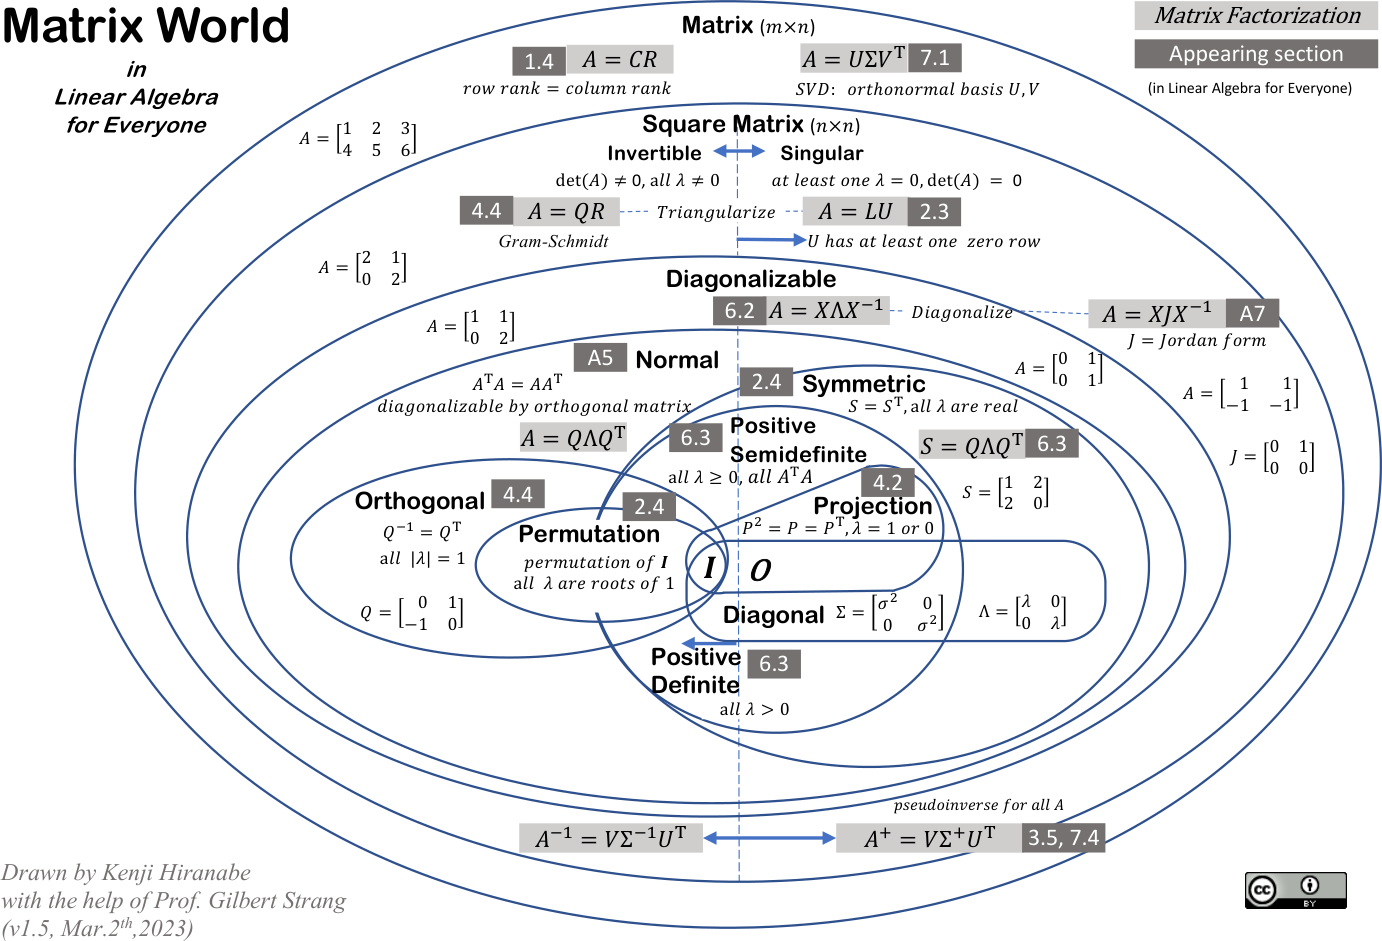
\includegraphics[width=\linewidth,height=0.6\textheight,keepaspectratio]{gfx/m2l3_hiranabe_fig1_matrix_world.png}
\par\smallskip{\small \textbf{Hình 1:} Thế giới Ma trận}
\end{figure}

\textbf{Các nhãn và chú thích trong biểu đồ Thế giới Ma trận:}

\begin{itemize}
  \item \textbf{Matrix World in Linear Algebra for Everyone:} Thế giới Ma trận trong ``Linear Algebra for Everyone''
  \item \textbf{Appearing section (Mục xuất hiện):} (in Linear Algebra for Everyone) (trong ``Linear Algebra for Everyone'')
  \item \textbf{Matrix Factorization:} Phân rã Ma trận
  \item \textbf{Matrix (m$\times$n):} Ma trận (m$\times$n)
\begin{itemize}
  \item $A = CR$ (1.4)
  \item $A = U\Sigma V^T$ (7.1)
  \item SVD: orthonormal basis \$U, V\$ (SVD: cơ sở trực chuẩn \$U, V\$)
  \item row rank = column rank (hạng hàng = hạng cột)
  \item pseudoinverse for all A (giả nghịch đảo cho mọi A): $A^+ = V\Sigma^+ U^T$ (3.5, 7.4)
\end{itemize}
  \item \textbf{Square Matrix (n$\times$n):} Ma trận vuông (n$\times$n)
  \item \textbf{Invertible:} Khả nghịch
\begin{itemize}
  \item det\$(A) \textbackslash{}neq 0\$, all $\lambda \neq 0$ (det\$(A) \textbackslash{}neq 0\$, mọi $\lambda \neq 0$)
  \item $A = QR$ (4.4)
  \item Gram-Schmidt
  \item $A^{-1} = V\Sigma^{-1} U^T$
\end{itemize}
  \item \textbf{Singular:} Suy biến
\begin{itemize}
  \item at least one $\lambda = 0$, det\$(A) = 0\$ (ít nhất một $\lambda = 0$, det\$(A) = 0\$)
  \item Triangularize (Tam giác hóa)
  \item $A = LU$ (2.3)
  \item $U$ has at least one zero row ($U$ có ít nhất một hàng không)
\end{itemize}
  \item \textbf{Diagonalizable:} Có thể chéo hóa
\begin{itemize}
  \item 6.2 $A = X\Lambda X^{-1}$
  \item Diagonalize (Chéo hóa)
  \item $A = XJX^{-1}$ (A7), $J =$ Jordan form ($J =$ dạng Jordan)
\end{itemize}
  \item \textbf{Normal:} Chuẩn (A5)
\begin{itemize}
  \item $A^T A = A A^T$
  \item diagonalizable by orthogonal matrix (có thể chéo hóa bằng ma trận trực giao)
  \item 6.3 $A = Q\Lambda Q^T$
\end{itemize}
  \item \textbf{Orthogonal:} Trực giao (4.4)
\begin{itemize}
  \item $Q^{-1} = Q^T$
  \item all $|\lambda| = 1$ (mọi $|\lambda| = 1$)
\end{itemize}
  \item \textbf{Permutation:} Hoán vị (2.4)
\begin{itemize}
  \item permutation of $I$ (hoán vị của $I$)
  \item all $\lambda$ are roots of \$1\$ (mọi $\lambda$ là căn của \$1\$)
\end{itemize}
  \item \textbf{Symmetric:} Đối xứng (2.4)
\begin{itemize}
  \item $S = S^T$, all $\lambda$ are real (mọi $\lambda$ là số thực)
\end{itemize}
  \item \textbf{Positive Semidefinite:} Nửa xác định dương
\begin{itemize}
  \item all $\lambda \ge 0$, all $A^T A$ (mọi $\lambda \ge 0$, mọi $A^T A$)
  \item $S = Q\Lambda Q^T$ (6.3)
\end{itemize}
  \item \textbf{Projection:} Chiếu (4.2)
\begin{itemize}
  \item $P^2 = P = P^T$, $\lambda = 1$ or \$0\$ ($\lambda = 1$ hoặc \$0\$)
\end{itemize}
  \item \textbf{Positive Definite:} Xác định dương (6.3)
\begin{itemize}
  \item all $\lambda > 0$ (mọi $\lambda > 0$)
\end{itemize}
  \item \textbf{Trung tâm biểu đồ:}
\begin{itemize}
  \item $I$: Identity (Đơn vị)
  \item $O$: ma trận không (zero matrix)
  \item Diagonal (Đường chéo) $\Sigma = \dots \Lambda = \dots$
\end{itemize}
  \item \textbf{Ghi chú góc dưới:}
\begin{itemize}
  \item Drawn by Kenji Hiranabe with the help of Prof. Gilbert Strang (v1.5, Mar.2th,2023) (Vẽ bởi Kenji Hiranabe với sự trợ giúp của GS. Gilbert Strang (v1.5, ngày 2 tháng 3 năm 2023))
\end{itemize}
\end{itemize}
